
\documentclass[12pt]{article}
\usepackage{amsfonts}
\usepackage{graphicx}

\newcommand{\real}{{\rm Re}}
\newcommand{\imag}{{\rm Im}}

\begin{document}

This document explains the history of the DeltaPA class that is the basis for the {\tt rmfit -r}
Faraday Rotation Measure refinement algorithm.  Two versions of the algorithm were implemented:
%
\begin{itemize}
\item Mark I - computes the phase of the complex-valued cross-correlation between Stokes $Q+iU$ profiles
\item Mark II - computes the phase of the inverse-variance weighted cross-correlation
\end{itemize}

The Mark I algorithm was first implemented in September 2006.   On 26 July 2007, the Mark II algorithm
replaced it.   On 6 April 2019, the code was reverted to Mark I after discovering a fundamental problem
with the Mark II algorithm, as explained in Sections 2 and 3 of this document.

\section{Mean value of position angle change \\ Mark I }

This section documents the propagation of error when estimating the
change in position angle, $\Delta\Psi$, between two polarization
profiles using the Mark I version of the algorithm implemented by {\tt rmfit -r}.
%
Let
\begin{equation}
P_k = Q_k + i U_k = L_k \exp i2\Psi_k
\end{equation}
represent the linear polarization of the $k$th phase bin in one profile and
\begin{equation}
P^\prime_k = Q^\prime_k + i U^\prime_k = L^\prime_k \exp i2\Psi^\prime_k
\end{equation}
the same in the other profile.  To find the mean value of $\Delta\Psi$,
\begin{equation}
\bar\Psi = {1\over N}\sum_{k=1}^N \Psi^\prime_k - \Psi_k
\end{equation}
use the cross-correlation
\begin{equation}
Z = \sum_{k=1}^N P^*_k P^\prime_k 
  = \sum_{k=1}^N L_k L^\prime_k \exp i2(\Psi^\prime_k - \Psi_k)
\end{equation}
such that
\begin{equation}
\bar\Psi
={1\over2}\tan^{-1}\left({\imag[Z]\over\real[Z]}\right).
\end{equation}
The variance of this estimate
\begin{equation}
\sigma_{\bar\Psi}^2 = \sum_{k=1}^N 
\left({\partial\bar\Psi\over\partial Q_k}\right)^2 \sigma_Q^2 +
\left({\partial\bar\Psi\over\partial U_k}\right)^2 \sigma_U^2 +
\left({\partial\bar\Psi\over\partial Q^\prime_k}\right)^2 \sigma_Q^{\prime2} +
\left({\partial\bar\Psi\over\partial U^\prime_k}\right)^2 \sigma_U^{\prime2}.
\label{eqn:var_Psi}
\end{equation}
To compute the partial derivatives, let
\begin{equation}
C = \real[Z] = \sum_{k=1}^N Q_kQ^\prime_k + U_kU^\prime_k,
\label{eqn:real_Z}
\end{equation}
\begin{equation}
S = \imag[Z] = \sum_{k=1}^N Q_kU^\prime_k - Q^\prime_kU_k,
\label{eqn:imag_Z}
\end{equation}
and
\begin{equation}
T = {S\over C},
\end{equation}
so that
\begin{equation}
{\partial\bar\Psi\over\partial Q_k} 
= {1\over1+T^2} \left( {U^\prime_k \over C} - {S Q^\prime_k\over C^2} \right)
= { C U^\prime_k - S Q^\prime_k \over C^2 + S^2 }
\end{equation}
Similarly
\begin{equation}
{\partial\bar\Psi\over\partial U_k} 
= { -C Q^\prime_k - S U^\prime_k \over C^2 + S^2 }
\end{equation}
\begin{equation}
{\partial\bar\Psi\over\partial Q^\prime_k} 
= { -C U_k - S Q_k \over C^2 + S^2 }
\end{equation}
\begin{equation}
{\partial\bar\Psi\over\partial U^\prime_k} 
= { C Q_k - S U_k \over C^2 + S^2 }
\end{equation}

The above equations have been tested over a range of signal to noise ratios, as shown in 
Figures~\ref{fig:mark1_error} and~\ref{fig:mark1_error_ratio}.  Everything looks good, except
down at low $S/N < 10$.

\begin{figure}
\centerline{\includegraphics[angle=-90,width=100mm]{plots/mark1_error.eps}}
\caption{\label{fig:mark1_error}
Standard deviation of 2500 RM estimates $\sigma_\mathrm{RM}$ as a function of signal-to-noise ratio $S/N$
using the Mark I implementation of RM refinement.  As expected, the noise scales as $(S/N)^{-1}$, as indicated
by the dashed line with a slope of -1.}
\end{figure}

\begin{figure}
\centerline{\includegraphics[angle=-90,width=100mm]{plots/mark1_error_ratio.eps}}
\caption{\label{fig:mark1_error_ratio}
Ratio between the mean estimated uncertainty $\epsilon_\mathrm{RM}$ and the standard deviation of 2500 RM estimates $\sigma_\mathrm{RM}$ as a function of signal-to-noise ratio $S/N$
using the Mark I implementation of RM refinement.  As expected, the ratio is approximately unity, as indicated
by the dashed line.}
\end{figure}

\section{Mean value of position angle change \\ Mark II}

This section documents the Mark II algorithm for estimating the change in
position angle, $\Delta\Psi$, and its uncertainty.  As before, let
\begin{equation}
P_k = Q_k + i U_k = L_k \exp i2\Psi_k
\end{equation}
represent the linear polarization of the $k$th phase bin in one profile and
\begin{equation}
P^\prime_k = Q^\prime_k + i U^\prime_k = L^\prime_k \exp i2\Psi^\prime_k
\end{equation}
the same in the other profile.  

Consider the {\bf weighted} cross-correlation,
$\bar{Z}=\bar{C}+i\bar{S}$, where $\bar C$ and $\bar S$ are the
weighted mean values of the real and imaginary components of
\begin{equation}
z_k = c_k + i s_k 
    = P^*_k P^\prime_k = L_k L^\prime_k \exp i2(\Psi^\prime_k - \Psi_k).
\end{equation}
That is, where
\begin{equation}
c_k = Q_kQ^\prime_k + U_kU^\prime_k,
\hspace{1cm}
s_k = Q_kU^\prime_k - U_kQ^\prime_k,
\label{eqn:ck_sk}
\end{equation}
and
\begin{eqnarray}
\sigma_{c_k}^2 & = &
 Q^{\prime2}_k\sigma_{Q_k}^2 + U^{\prime2}_k\sigma_{U_k}^2 +
 Q^2_k\sigma_{Q^\prime_k}^2 + U^2_k\sigma_{U^\prime_k}^2 \label{eqn:var_ck} \\
\sigma_{s_k}^2 & = &
 U^{\prime2}_k\sigma_{Q_k}^2 + Q^{\prime2}_k\sigma_{U_k}^2 +
 U^2_k\sigma_{Q^\prime_k}^2 + Q^2_k\sigma_{U^\prime_k}^2 \label{eqn:var_sk} \\
\sigma_{s_k c_k} & = &
 Q^\prime_k U^\prime_k (\sigma_{Q_k}^2 - \sigma_{U_k}^2) +
 Q_kU_k (\sigma_{U^\prime_k}^2 -\sigma_{Q^\prime_k}^2)
\label{eqn:covar_ck_sk}
\end{eqnarray}
the weighted means and their variances and covariance are given by
\begin{equation}
\bar C = \sigma_{\bar C}^2 \sum_{k=1}^N { c_k \over \sigma_{c_k}^2 }
\hspace{1cm}
\bar S = \sigma_{\bar S}^2 \sum_{k=1}^N { s_k \over \sigma_{s_k}^2 }
\label{eqn:barC_barS}
\end{equation}
and
\begin{equation}
\sigma_{\bar C}^2 = \left[ \sum_{k=1}^N{1\over\sigma_{c_k}^2} \right]^{-1}
\hspace{5mm}
\sigma_{\bar S}^2 = \left[ \sum_{k=1}^N{1\over\sigma_{s_k}^2} \right]^{-1}
\hspace{5mm}
\sigma_{\bar S \bar C} = \sum_{k=1}^N
\left[\sigma_{\bar S}\sigma_{\bar C}\over\sigma_{s_k}\sigma_{c_k}\right]^2
                         \sigma_{s_k c_k}
\label{eqn:var_covar_barC_barS}
\end{equation}

\noindent
The expectation value of $\Delta\Psi=\Psi^\prime_k - \Psi_k$ is given by
\begin{equation}
\langle\Delta\Psi\rangle
={1\over2}\tan^{-1}\left({\bar S\over\bar C}\right).
\end{equation}
and the variance of the expectation value
\begin{equation}
{\mathrm{var}}(\langle\Delta\Psi\rangle) = 
{ \bar C^2\sigma_{\bar S}^2 + \bar S^2\sigma_{\bar C}^2
  + 2 \bar S\bar C \sigma_{\bar S \bar C} \over 
  \left(\bar C^2 + \bar S^2\right)^2 }
\label{eqn:var_delta_Psi}
\end{equation}

The above equations have been tested over a range of signal to noise ratios, as shown in
Figures~\ref{fig:mark2_error} and~\ref{fig:mark2_error_ratio}.  These plots show that
the Mark II algorithm

\begin{enumerate}
\item slightly underestimates the uncertainty of $RM$ estimates; and 
\item more importantly, fails to exploit $S/N$ as expected.
\end{enumerate}

\begin{figure}
\centerline{\includegraphics[angle=-90,width=100mm]{plots/mark2_error.eps}}
\caption{\label{fig:mark2_error}
Standard deviation of 2500 RM estimates $\sigma_\mathrm{RM}$ as a function of signal-to-noise ratio $S/N$
using the Mark II implementation of RM refinement.  The dashed line has a slope of -1, as expected when
the error scales as $(S/N)^{-1}$.  The Mark II algorithm clearly fails to produce estimates with the expected
uncertainty; at the highest $S/N$, the standard deviation is over ten times the predicted value.}
\end{figure}

\begin{figure}
\centerline{\includegraphics[angle=-90,width=100mm]{plots/mark2_error_ratio.eps}}
\caption{\label{fig:mark2_error_ratio}
Ratio between the mean estimated uncertainty $\epsilon_\mathrm{RM}$ and the standard deviation of 2500 RM estimates $\sigma_\mathrm{RM}$ as a function of signal-to-noise ratio $S/N$
using the Mark II implementation of RM refinement.  The dashed line indicates the expected ratio of unity;
the Mark II algorithm tends to underestimate uncertainty.}
\end{figure}


\section{The Problem With Mark II}

Consider the special case when the two profiles are identical,
i.e. $P_k^\prime = P_k$, with equal noise in all Stokes parameters, 
i.e. $\sigma_{Q_k}=\sigma_{U_k}=\sigma_{Q^\prime_k}=\sigma_{U^\prime_k}=\sigma$.
In this case, referring to Equations~\ref{eqn:var_ck} to~\ref{eqn:covar_ck_sk},
$\sigma^2_{c_k}=\sigma^2_{s_k}=2\sigma^2 L_k^2$ and $\sigma_{s_k c_k}=0$.
%
Referring to Equation \ref{eqn:var_covar_barC_barS}, the variance of the weighted
mean cosine and sine,
\begin{equation}
\sigma_{\bar C}^2 = \sigma_{\bar S}^2 = 2\sigma^2 \left[ \sum_{k=1}^N{1\over L_k^2} \right]^{-1}.
\end{equation}
%
Substitution of the above into Equation~\ref{eqn:barC_barS} yields
\begin{equation}
\bar C = \sum_{k=1}^N { c_k \over L_k^2 } \left[ \sum_{k=1}^N { 1 \over L_k^2 } \right]^{-1}
\hspace{1cm}
\bar S = \sum_{k=1}^N { s_k \over L_k^2 } \left[ \sum_{k=1}^N { 1 \over L_k^2 } \right]^{-1}
\end{equation}

Already, the problem is apparent.  The above equations represent weighted averages in which each cross-correlation
$c_k$ and $s_k$ are weighted by the {\bf inverse} of the linearly polarized flux $L^2$.  Such a weighted average
gives less weight to the samples with greater linearly polarized flux!  This is opposite to what is intended,
and is a consqeuence of sticking too blindly to the rules of first-order linear error propagation.

Also, in the special case that $P_k^\prime = P_k$, then (referring to Equation~\ref{eqn:ck_sk}) 
$c_k=L^2$, $s_k=0$, $\bar S = 0$, and
\begin{equation}
\bar C = N \left[ \sum_{k=1}^N{1\over L_k^2} \right]^{-1}.
\end{equation}
%
Finally, plugging everything into Equation~\ref{eqn:var_delta_Psi} yields
\begin{equation}
{\mathrm{var}}(\langle\Delta\Psi\rangle) = 2 {\sigma^2 \over N^2} \sum_{k=1}^N{1\over L_k^2}.
\end{equation}
%
At first glance, it may seem reasonable that the variance of the weighted mean position angle change
should be inversely proportional to the square of the linearly polarized flux.  However, it is proportional
to the sum of terms that are inversely proportional to the square of the linearly polarized flux.
Adding more detectable phase bins increases $N$ (thereby decreasing the variance, as expected) but also adds more terms 
to this sum (thereby {\bf increasing} the variance!)

By increasing the $S/N$, we increase each of the $L_k$ terms and decrease the variance of the weighted mean position angle change; however, we also increase the number of phase bins that are detected above the noise and increase the sum in the above equation.  This effect stops the standard deviation of RM estimates from scaling as one over $S/N$.  

\subsubsection{Revisiting the Mark I Implementation}

As written, it is not possible to compute the sums in Equations~\ref{eqn:var_Psi}
through~\ref{eqn:imag_Z} in a single loop.  After grouping like terms,
%
\begin{equation}
\sigma_{\bar\Psi}^2 =
(C^2+S^2)^{-2} \left(C^2 \sigma_S^2 + S^2 \sigma_C^2 - 2 CS \sigma_{CS} \right)
\label{eqn:var_Psi_simplified}
\end{equation}
%
where
\begin{equation}
\sigma_C^2 = \sum_{k=1}^N \sigma_{c_k}^2
\hspace{5mm}
\sigma_S^2 = \sum_{k=1}^N \sigma_{s_k}^2 
\hspace{5mm}
\sigma_{CS} = \sum_{k=1}^N \sigma_{s_k c_k}
\label{eqn:var_covar_C_S}
\end{equation}

\end{document}
